% \documentclass[draft=True]{thesis}
% \usepackage[margin=0.5in]{geometry}
% \usepackage{graphicx, slashed, siunitx}
% \usepackage[utf8]{inputenc}
% \usepackage{xr-hyper}
% \documentclass[a4paper,10pt,draft]{thesis}
\usepackage{physics,amsmath, amsfonts, siunitx, amssymb, graphicx, slashed,subcaption}
\usepackage[utf8]{inputenc}
\usepackage[margin=1in]{geometry}
\usepackage[hidelinks]{hyperref}
\usepackage{xr-hyper}
\newcommand{\n}[1]{\nu_{#1}}
\newcommand{\na}{\nu_\alpha}
\newcommand{\nb}{\nu_\beta}
\newcommand{\ana}{\bar{\nu}_\alpha}
\newcommand{\an}[1]{\bar{\nu}_{\text{#1}}}
\newcommand{\anb}{\bar{\nu}_\beta}
\renewcommand{\a}{\alpha}
\renewcommand{\b}{\beta}
\newcommand{\ab}{\alpha\beta}


\renewcommand{\ne}{\nu_e}
\newcommand{\nm}{\nu_\mu}
\newcommand{\nt}{\nu_\tau}
\newcommand{\ns}{\nu_s}

\newcommand{\ane}{\bar{\nu}_e}
\newcommand{\anm}{\bar{\nu}_\mu}
\newcommand{\ant}{\bar{\nu}_\tau}
\newcommand{\ans}{\bar{\nu}_s}

\newcommand{\nee}{\nu_e \to \nu_e}
\newcommand{\nem}{\nu_e \to \nu_\mu}
\newcommand{\net}{\nu_e \to \nu_\tau}
\newcommand{\nes}{\nu_e \to \nu_s}

\newcommand{\nme}{\nu_\mu \to \nu_e}
\newcommand{\nmm}{\nu_\mu \to \nu_\mu}
\newcommand{\nmt}{\nu_\mu \to \nu_\tau}
\newcommand{\nms}{\nu_\mu \to \nu_s}



\newcommand{\Pee}{P_{e  e}}
\newcommand{\Pem}{P_{e  \mu}}
\newcommand{\Pet}{P_{e  \tau}}
\newcommand{\Pes}{P_{e  s}}

\newcommand{\Pme}{P_{\mu  e}}
\newcommand{\Pmm}{P_{\mu\mu}}
\newcommand{\Pmt}{P_{\mu  \tau}}
\newcommand{\Pms}{P_{\mu  s}}


\newcommand{\Pte}{P_{P_{\tau e}}}
\newcommand{\Ptm}{P_{\tau  \mu}}
\newcommand{\Ptt}{P_{\tau  \tau}}
\newcommand{\Pts}{P_{\mu  s}}

\newcommand{\Paeae}{P_{\bar{e}  \bar{e}}}
\newcommand{\Paeam}{P_{\bar{e}  \bar{\mu}}}
\newcommand{\Paeat}{P_{\bar{e}  \bar{\tau}}}
\newcommand{\Paeas}{P_{\bar{e}  \bar{s}}}

\newcommand{\Pamae}{P_{\bar{\mu}  \bar{e}}}
\newcommand{\Pamam}{P_{\bar{\mu}  \bar{\mu}}}
\newcommand{\Pamat}{P_{\bar{\mu}  \bar{\tau}}}
\newcommand{\Pamas}{P_{\bar{\mu}  \bar{s}}}


\newcommand{\Patae}{P_{\bar{\tau}  \bar{e}}}
\newcommand{\Patam}{P_{\bar{\tau}  \bar{\mu}}}
\newcommand{\Patat}{P_{\bar{\tau}  \bar{\tau}}}
\newcommand{\Patas}{P_{\bar{\mu}  \bar{s}}}

\renewcommand{\th}[1][]{%
  \theta\ifx\\#1\\\else_\text{#1}\fi
}
\newcommand{\thm}[1][]{%
  \theta^\text{M}\ifx\\#1\\\else_\text{#1}\fi
}
\renewcommand{\t}[1]{\text{{#1}}}
\newcommand{\avg}[1]{\left\langle {#1} \right \rangle}
\newcommand*{\dm}[1][]{%
  \Delta m^2\ifx\\#1\\\else_\text{#1}\fi
}
\newcommand{\zreco}{\cos{(\theta_z^{reco})}}
\newcommand{\ztrue}{\cos{(\theta_z^{true})}}
\newcommand{\z}{\cos{(\theta_z)}}
\newcommand{\Ereco}{E^{reco}}
\newcommand{\Etrue}{E^{true}}
\newcommand{\Aeff}{A^\text{eff}}
\newcommand{\emm}{\epsilon_{\mu\mu}}
\newcommand{\emt}{\epsilon_{\mu\tau}}
\newcommand{\eet}{\epsilon_{e\tau}}
\newcommand{\eem}{\epsilon_{e\mu}}
\newcommand{\ett}{\epsilon_{\tau\tau}}
\newcommand{\ep}{\epsilon^\prime}

% \begin{document}
\section{Non-Standard Interactions}\label{sec:nsiResults}
\subsection{Constraining the NSI parameters}\label{sec:constraining}
In this section, we will constrain the four NSI parameters $\ett$, $\emt$, $\eem$, and $\eet$ by considering the detectors separately as well as jointly.
For our analyses, we define our $\chi^2$ as
\begin{align} \label{eq:chisq}
    \chi^{2}(\hat{\theta},\alpha,\beta, \kappa)=\sum_{ijk} \frac{\left(N^\text{th}-N^\text{data}\right)_{ijk}^{2}}
    {\left(\sigma^\text{data}_{ijk}\right)^{2} + \left(\sigma^\text{syst}_{ijk}\right)^{2}}+ 
    \frac{(1-\alpha)^2}{\sigma_\alpha^2} + \frac{\beta^2}{\sigma_\beta^2}\,
\end{align}
where we minimize over the model parameters $\hat{\theta} \in \{\dm, \theta_{23}, \epsilon\}$, the penalty terms $\alpha$ and $\beta$, and the free parameter $\kappa$.
$N_{ijk}^\text{th}$ is the expected number of events from theory, and $N_{ijk}^\text{data}$ is the observed number of events in that bin. 

In our simulations of $N_{ijk}^\text{th}$, we set all standard oscillation parameters to their current best-fit values of Eq.~\ref{eq:PINGUparams}, 
except for $\dm$ and $\theta_{23}$
which we vary over their $3\sigma$ limits \SIrange{2.435e-3}{2.598e-3}{\eV \squared} and \SIrange{40.1}{51.7}{\degree}, respectively.

We set $\sigma_\alpha = 0.25$ as the atmospheric flux normalization error, and $\sigma_\beta = 0.04$ as the zenith angle slope error~\cite{hondapaper}. 
The observed event number has an associated Poissonian uncertainty $\sigma_{ijk}^\text{data} = \sqrt{N_{ijk}^\text{data}}$.
For IceCube, the event count takes the form
\begin{align}
    N^\text{th}_{ij} = \alpha\left[1+\beta (0.5 + \zreco_i )\right] N_{ij}(\hat{\theta})\,,
\end{align}
with $N_{ij}(\hat{\theta})$ from Eq.~\ref{eq:ICevents}. Here, we allow the event distribution to rotate around the median cosine-zenith of $\zreco = -0.5$.

For DeepCore and PINGU, and the event count takes the form
\begin{align}
    N^\text{th}_{ijk} = \alpha\left[1+\beta \zreco_i \right] N_{ijk}(\hat{\theta}) + \kappa N_{ijk}^{\mu_{atm}}\,,
\end{align}
with $N_{ijk}(\hat{\theta})$ from Eq.~\ref{eq:MCevents}. $N_{ijk}^{\mu_{atm}}$ is the muon background, which is left to float freely in the DeepCore analysis.
The background at PINGU can be considered negligible to first order~\cite{PINGUdata}, and we thus put $\kappa=0$ when calculating the PINGU $\chi^2$.
For DeepCore and PINGU, the median cosine-zenith is $\zreco = 0$, and we allow the event count to rotate around this point.

We treat the uncorrelated systematic uncertanties differently for each detector. For IceCube, we set $\sigma_{ijk}^\text{syst} = f\sqrt{N_{ijk}^\text{data}}$.
We consider best, normal, and worst-case scenarios in IceCube using
$f=5\%$, $10\%$, and $15\%$ respectively. For PINGU, we use the same form but instead use $f=0\%$, $3\%$, and $5\%$. %TODO: maybe source/justification for these values?
For DeepCore, we use the provided systematic error distribution which accounts for uncertainties in the finite MC statistics and the data-driven 
muon background estimate~\cite{DC2019data}. This is summarized in Table~\ref{table:syst_errors}.  %TODO segue
{\renewcommand{\arraystretch}{1.2}
\begin{table}
   \begin{tabular}{lccc}
      \hline \hline
      Experiment & Best case & Baseline & Worst case \\
      \hline
      IceCube & $5\%$ & $10\%$ & $15\%$ \\
      PINGU & $0\%$ & $3\%$ & $5\%$ \\
      \hline \hline
   \end{tabular}
   \caption{Our definition of the best, baseline, and worst case scenarios considered in each experiment, modelled by $\sigma_{ijk}^\text{syst} = f\sqrt{N_{ijk}^\text{data}}$ with $f$ from the table.
   We do not consider different DeepCore scenarios because her systematic error distribution is already provided in the data release~\cite{DC2019data}.}\label{table:syst_errors}
\end{table}

For the joint analysis, we follow the parameter goodness-of-fit prescription~\cite{maltoni2003} and construct the joint $\chi^2$ as 
\begin{align}\label{eq:joint_chisq}
    \chi^2_\text{joint} = \sum_\text{exp}\chi^2_\text{exp} - \chi^2_\text{exp,min}\,
\end{align}
with test statistic $\chi^2_\text{joint,min}$. The $\Delta \chi^2_\text{joint}$ is then $\Delta \chi^2_\text{joint} = \chi^2_\text{joint} - \chi^2_\text{joint,min}$.

After the oscillation parameters have been marginalized out, we plot $\Delta \chi^2$ for each of the four NSI parameters in Fig.~\ref{fig:3D_NO}. 
The results are shown in Fig.~\ref{fig:IC_3D} and summarized in Tables~\ref{table:IC_DC_results} and~\ref{table:PINGU_joint_results}.

Comparing the PINGU and the DeepCore results in Fig.~\ref{fig:3D_NO}, we note that the best-fit for each NSI parameter for the PINGU experiment is expected to be zero. This is because the `data' we generated during 
the PINGU simulations assume no NSI since they have yet to be observed in nature. This introduces a non-NSI bias in all joint analyses which include PINGU,
since PINGU has stronger statistics than DeepCore and will thus pull the joint $\chi^2$ towards $\epsilon =0$.

\begin{figure}
   \begin{center}
      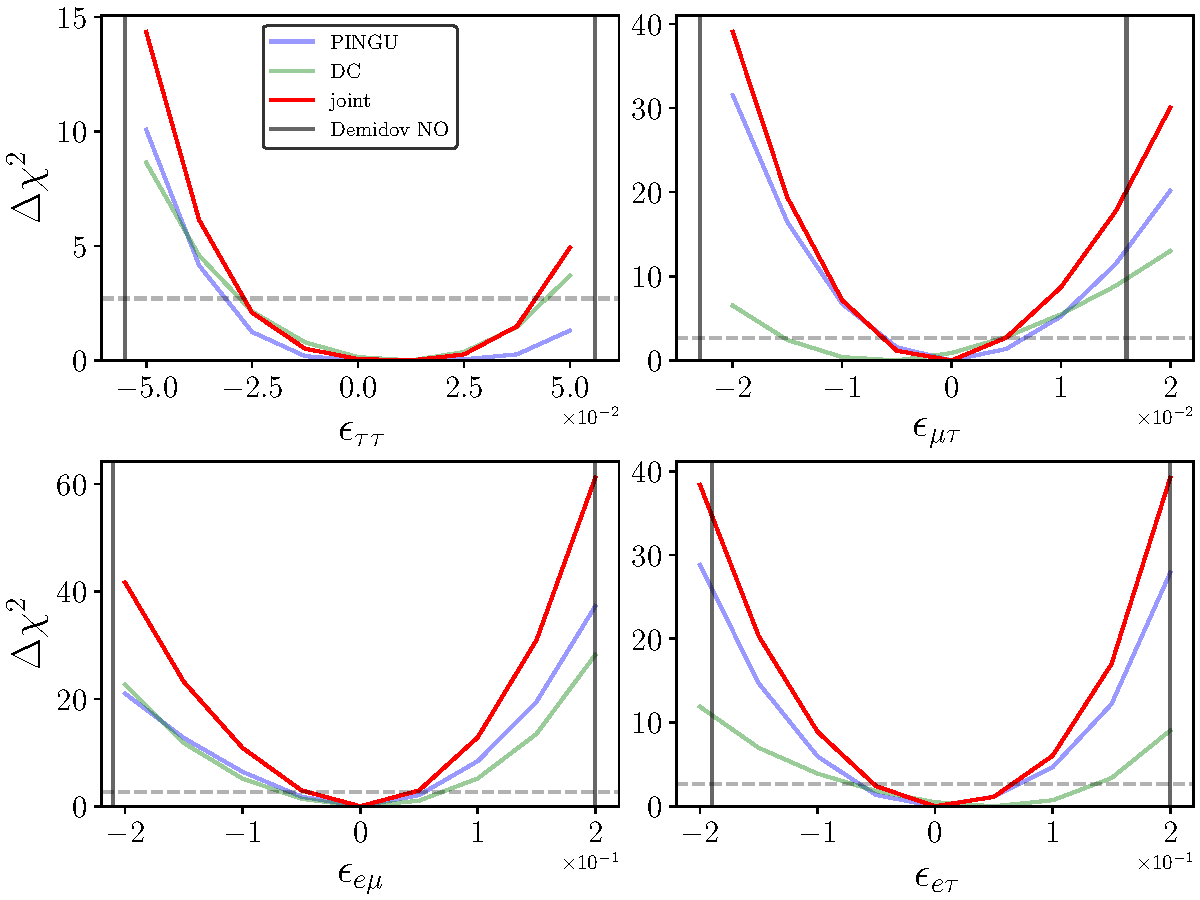
\includegraphics[width=0.6\textwidth]{figures/joint_3D_NO.pdf}
      \caption{PINGU and DeepCore best-case scenario, with their joint $\Delta \chi^2$ in black. $\dm$ and $\theta_{23}$ and have been marginalized out, and all other NSI 
      parameters not shown in each panel are fixed to zero. 
      IceCube tracks only reveal $\emt$, and are displayed separately in Fig.~\ref{fig:IC_3D}.}\label{fig:3D_NO}
   \end{center}
\end{figure} 
\begin{figure}
   \begin{center} 
      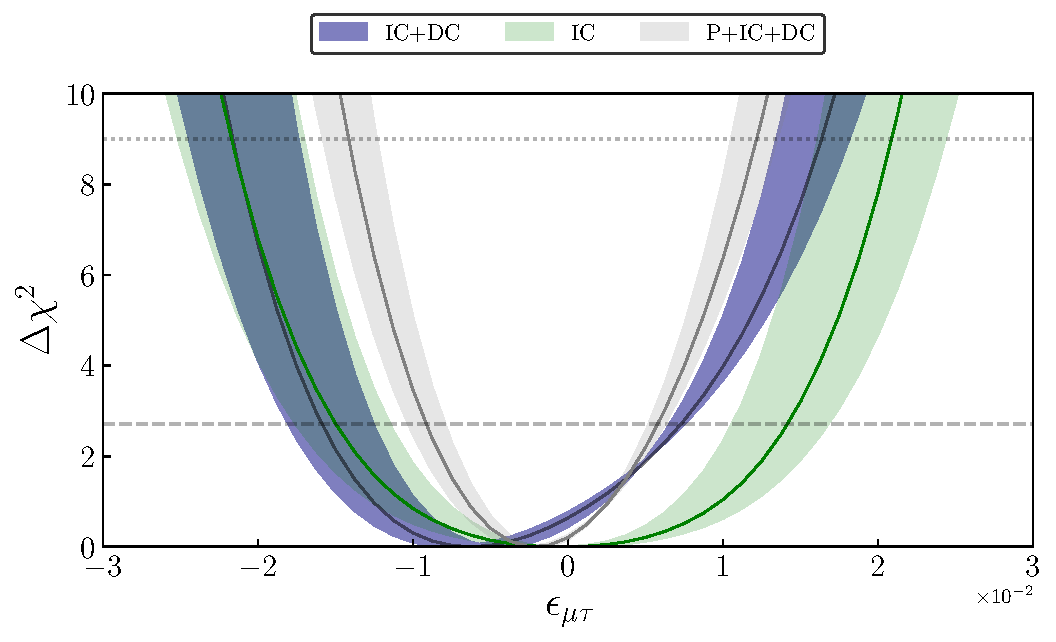
\includegraphics[width=0.6\textwidth]{figures/PID_3D_emt.pdf}
      \caption{$\emt$ $\Delta \chi^2$ regions for scenarios as defined in Table~\ref{table:syst_errors}.
    $\dm$ and $\theta_{23}$ and have been marginalized out, and all other NSI 
    parameters other than $\emt$ are fixed to zero.}\label{fig:IC_3D}
   \end{center}
\end{figure}



{\renewcommand{\arraystretch}{1.3}
 \begin{table}
   \begin{center}
   \begin{tabular}{lcccccc}
      \hline \hline
      Parameter & Best 90\% CL & Best $3\sigma$& Baseline 90\% CL & Baseline $3\sigma$ & Worst 90\% CL & Worst $3\sigma$\\
      \hline & \multicolumn{6}{c}{IceCube}  \\
      $\emt$ &  [-0.008, 0.009] &  [-0.014, 0.017] &   [-0.009, 0.01] &  [-0.015, 0.018] &   [-0.01, 0.011] &   [-0.017, 0.02] \\\\
      & \multicolumn{6}{c}{DeepCore}\\ [0.3em]
      $\ett$ &  [-0.044, 0.051] &  [-0.062, 0.069] &  [-0.046, 0.054] &         [-0.065] &  [-0.049, 0.057] &          [-0.07] \\
      $\emt$ &  [-0.008, 0.009] &  [-0.014, 0.017] &   [-0.009, 0.01] &  [-0.015, 0.018] &   [-0.01, 0.011] &   [-0.017, 0.02] \\
      $\eem$ &  [-0.079, 0.081] &   [-0.16, 0.14] &  [-0.11, 0.094] &  [-0.20, 0.16] &   [-0.14, 0.11] &   [-0.23, 0.18] \\
      $\eet$ &  [-0.079, 0.098] &  [-0.15, 0.16] &   [-0.10, 0.11] &  [-0.19, 0.18] &  [-0.13, 0.13] &  [-0.23, 0.12] \\\\
      &\multicolumn{6}{c}{IceCube + DeepCore}\\
      $\emt$ &  [-0.029, 0.007] &          [0.026] &  [-0.029, 0.007] &          [0.026] &  [-0.029, 0.007] &          [0.026] \\
      \hline
      \hline
   \end{tabular}
   \end{center}
   \caption{IceCube and DeepCore results from the $\Delta \chi^2$ in Fig.~\ref{fig:IC_3D}. Best, baseline, and worst refer to 
   the systematic uncertainty scenarios considered as in Table~\ref{table:syst_errors}.}\label{table:IC_DC_results}
\end{table}
\begin{table}
   \begin{tabular}{lcccccc}
      \hline \hline
      Parameter & Best 90\% CL & Best $3\sigma$& Baseline 90\% CL & Baseline $3\sigma$ & Worst 90\% CL & Worst $3\sigma$\\
      \hline & \multicolumn{6}{c}{PINGU} \\
      $\ett$ &  [-0.054, 0.067] &               [] &  [-0.054, 0.067] &               [] &  [-0.054, 0.067] &               [] \\
      $\emt$ &  [-0.029, 0.007] &          [0.026] &  [-0.029, 0.007] &          [0.026] &  [-0.029, 0.007] &          [0.026] \\
      $\eem$ &  [-0.12, 0.15] &  [-0.23, 0.24] &  [-0.12, 0.15] &  [-0.23, 0.24] &  [-0.12, 0.15] &  [-0.23, 0.24] \\
      $\eet$ &   [-0.084, 0.15] &  [-0.19, 0.21] &   [-0.084, 0.15] &  [-0.19, 0.21] &   [-0.084, 0.15] &  [-0.19, 0.21] \\\\
      & \multicolumn{6}{c}{DeepCore + PINGU} \\
      $\ett$ &  [-0.036, 0.046] &  [-0.056, 0.064] &  [-0.038, 0.048] &  [-0.058, 0.067] &   [-0.039, 0.05] &          [-0.06] \\
      $\emt$ &  [-0.009, 0.006] &  [-0.015, 0.013] &   [-0.01, 0.006] &  [-0.016, 0.014] &  [-0.011, 0.007] &  [-0.017, 0.015] \\
      $\eem$ &   [-0.06, 0.077] &  [-0.126, 0.127] &  [-0.071, 0.086] &  [-0.149, 0.141] &  [-0.082, 0.097] &  [-0.17, 0.16] \\
      $\eet$ &  [-0.052, 0.095] &  [-0.112, 0.144] &  [-0.061, 0.103] &  [-0.131, 0.155] &  [-0.067, 0.11] &  [-0.15, 0.17] \\\\
      & \multicolumn{6}{c}{IceCube + DeepCore + PINGU}  \\
      $\emt$ &  [-0.009, 0.006] &  [-0.015, 0.013] &   [-0.01, 0.006] &  [-0.016, 0.014] &  [-0.011, 0.007] &  [-0.017, 0.015] \\
      \hline
      \hline
   \end{tabular}
   \caption{PINGU and joint results from the $\Delta \chi^2$ in Fig.~\ref{fig:3D_NO}. Best, baseline, and worst refer to 
   the systematic uncertainty scenarios considered as in Table~\ref{table:syst_errors}.}\label{table:PINGU_joint_results}
\end{table}

\begin{table}
   \begin{center}
   \begin{tabular}{lccc}
           \hline \hline & \multicolumn{3}{c} {\text {Best fit}} \\
           \cline { 2 - 4 } Parameter & $\dm$ & $\theta_{23}$  & $\epsilon$  \\
           \hline \multicolumn{3}{c} {\hspace{2.5cm} DeepCore }  \\[0.1em]
           $\ett$ &  2.435 & 47.84 & 0.0125 \\
           $\emt$ &  2.435 & 43.97 & -0.005 \\
           $\eem$ &  2.435 & 43.97 & 0 \\
           $\eet$ &  2.435 & 43.97  & 0.05 \\\\
           \multicolumn{3}{c} {\hspace{2.5cm} IceCube } \\
           $\emt$ &  2.435 & 51.70 & 0 \\
           \multicolumn{3}{c} {\hspace{2.5cm} IceCube + DeepCore } \\
           $\emt$ &  2.517 & 43.97 & -0.01 \\
           \hline
           \hline
   \end{tabular}
   \end{center}
   \caption{Best fit points for $\dm$ and $\theta_{23}$ are given in units of $\si{10^{-3}\eV\squared}$ and
   degrees, respectively.}\label{table:bestfit}
\end{table}
\newpage


 \begin{figure}[t]
   \begin{center}
      \begin{subfigure}{0.38\textwidth}
         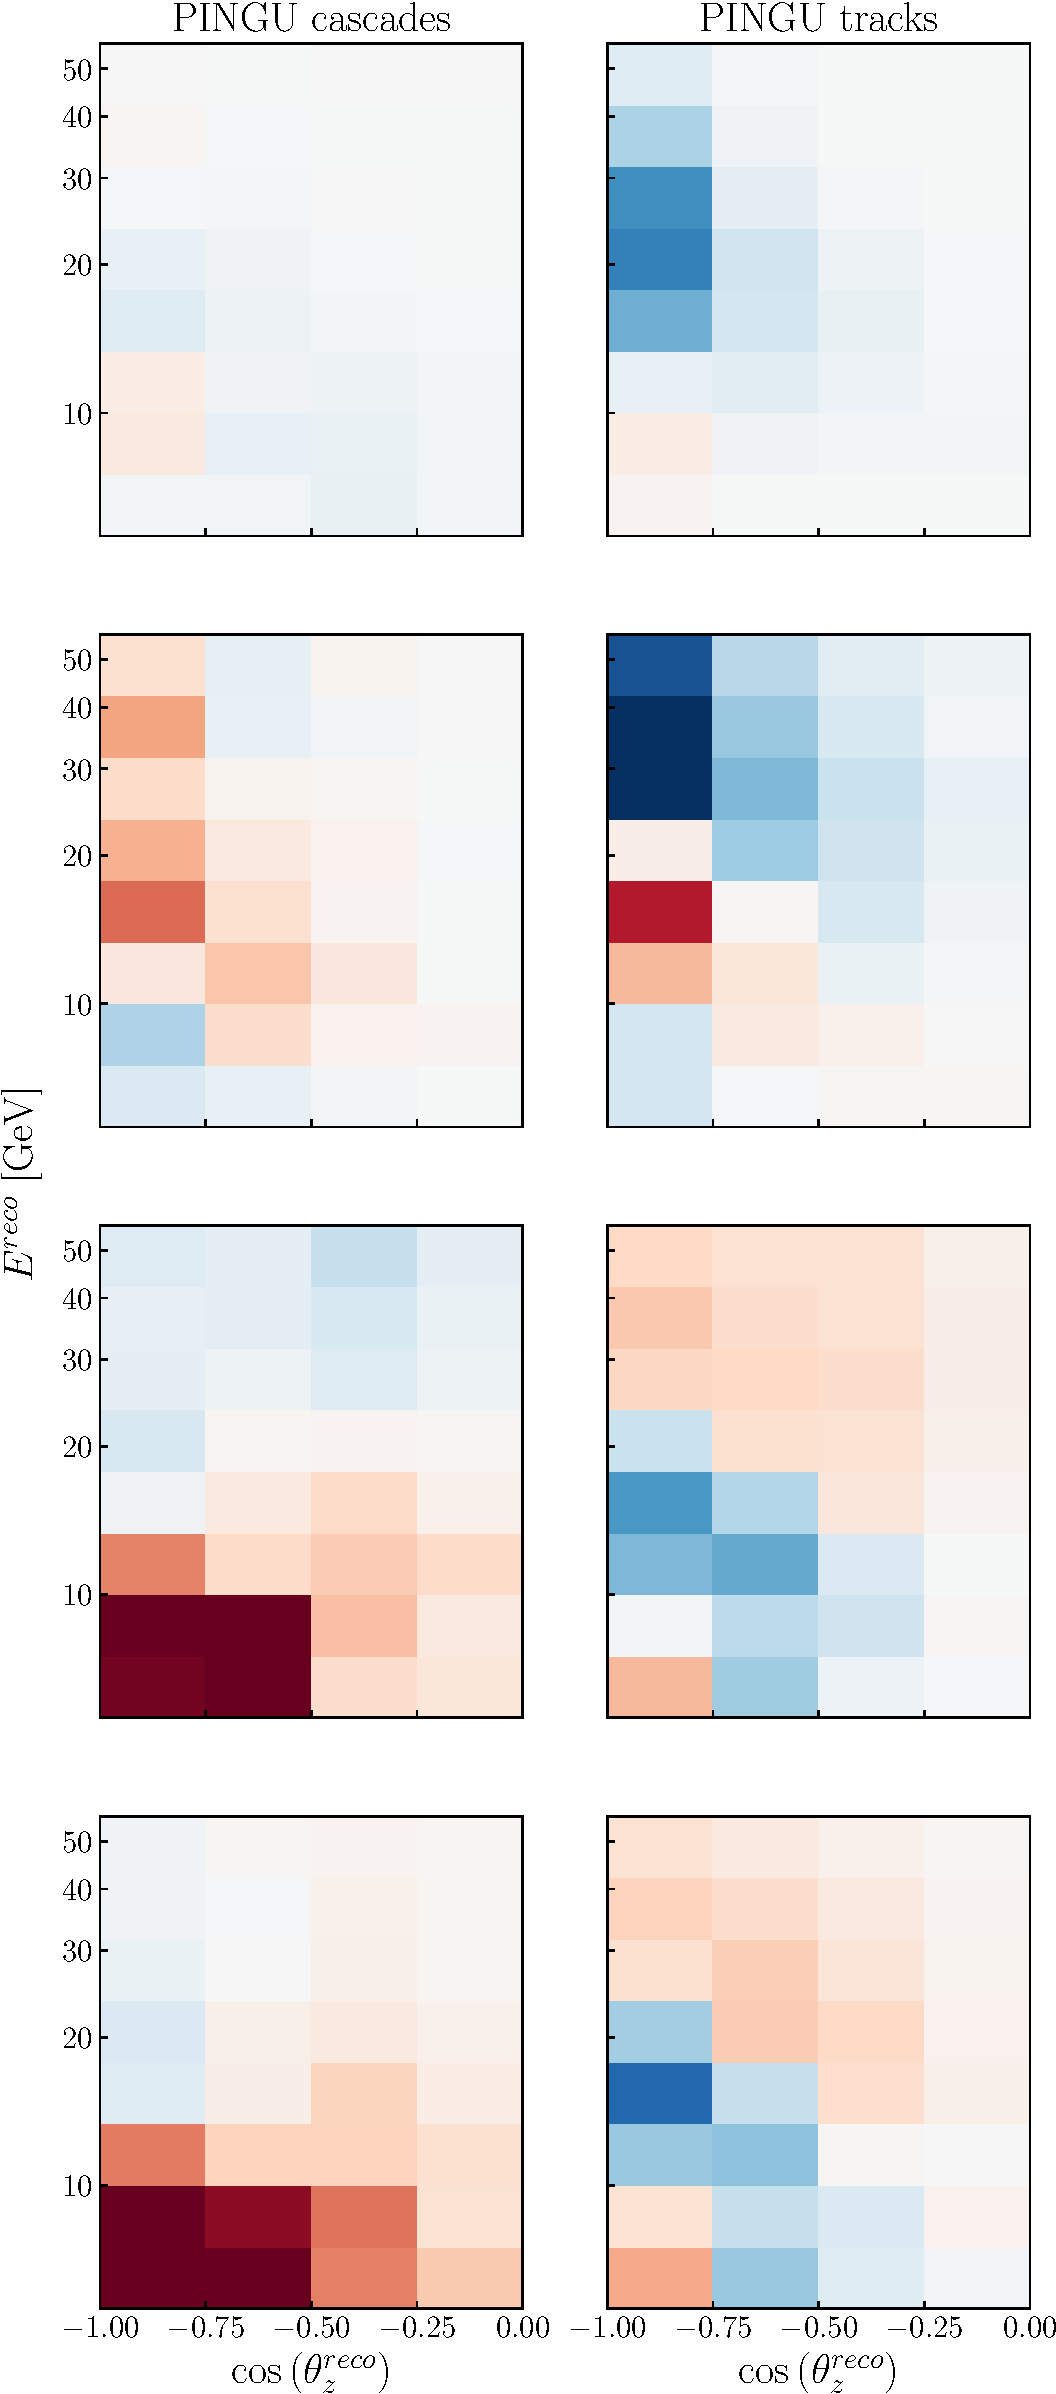
\includegraphics[width=1\linewidth]{figures/PINGU_event_pulls.pdf}
         \caption{PINGU}\label{fig:PINGU_event_pulls}
      \end{subfigure}
      \begin{subfigure}{0.4\textwidth}
         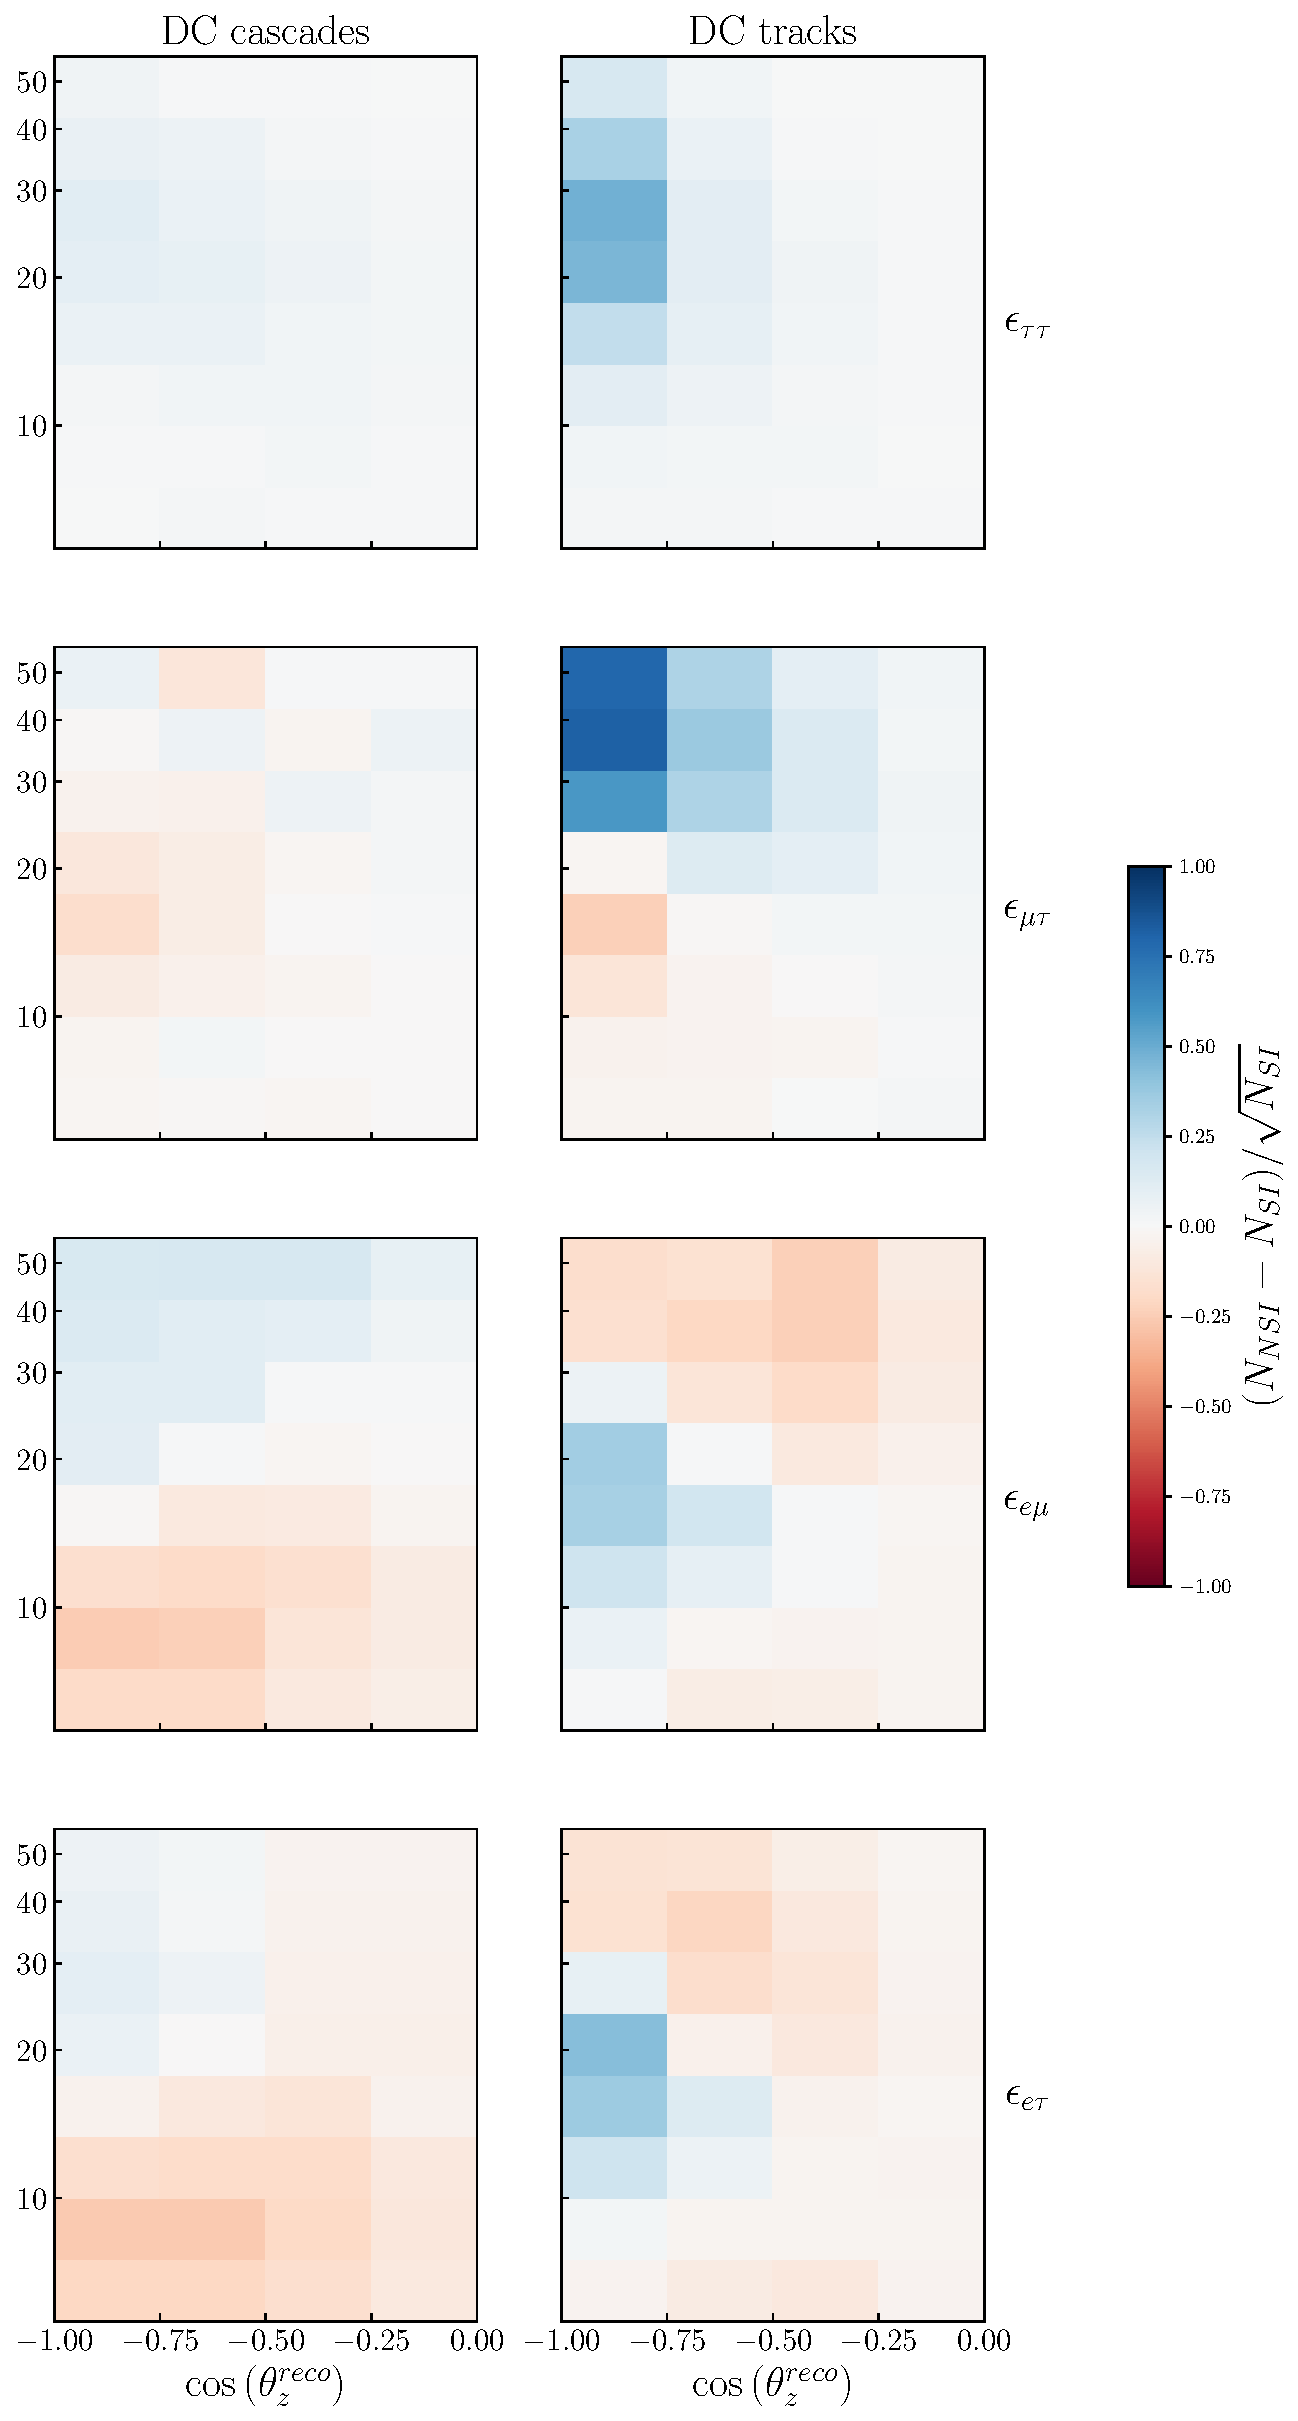
\includegraphics[width=1\linewidth]{figures/DC_event_pulls.pdf}
         \caption{DeepCore}\label{fig:DC_event_pulls}
      \end{subfigure}
    \end{center}
   \caption{Expected pulls of the form $(N_{NSI} - N_{SI})/\sqrt{N_{SI}}$ for PINGU and DeepCore after 3 years.}\label{fig:event_pulls} 
\end{figure}%TODO: redo these with same emt as flux_ratio? keep this, but align them better



%TODO: subsection about comparison between different papers. 

\begin{figure}
   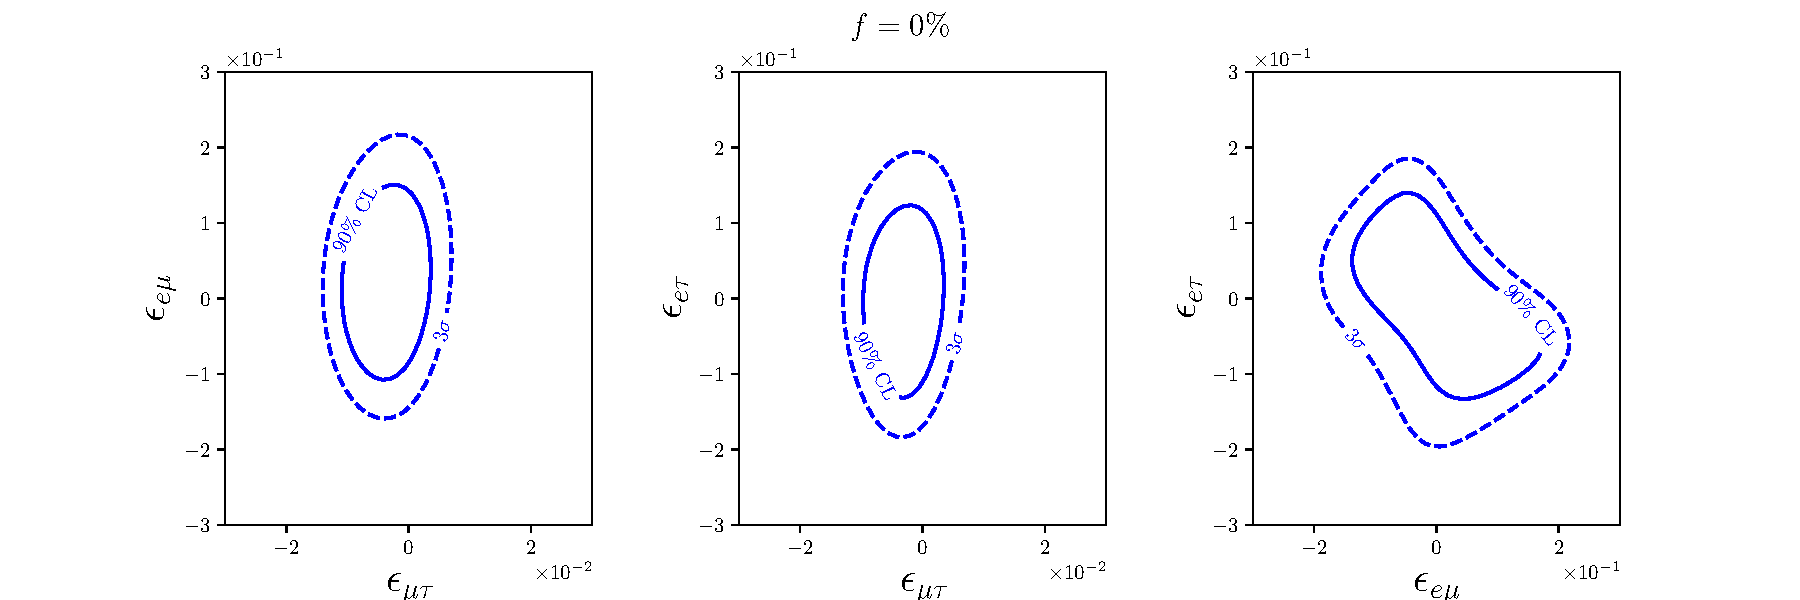
\includegraphics[width=0.9\textwidth]{figures/PINGU_2D_all_f0.pdf}
\end{figure}
\begin{figure}
   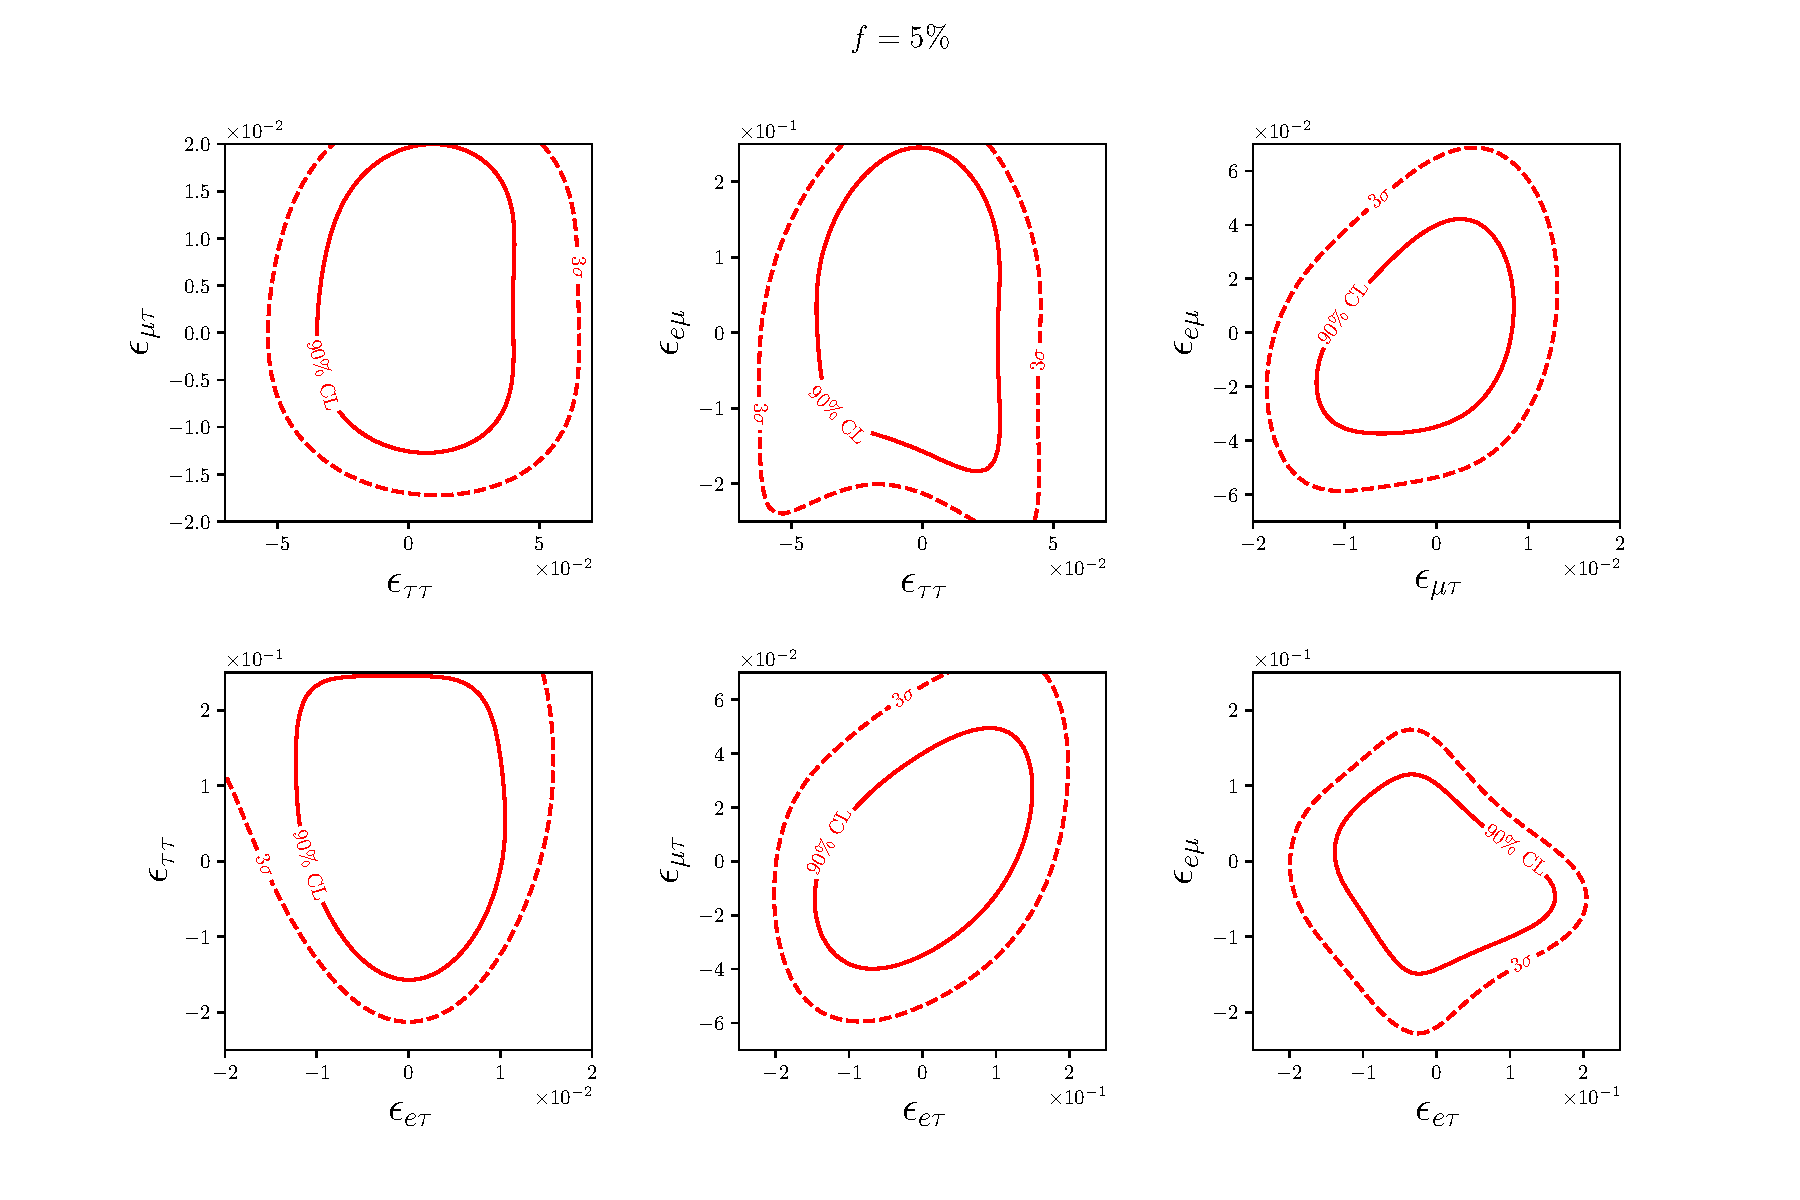
\includegraphics[width=0.9\textwidth]{figures/PINGU_2D_all_f5.pdf}
\end{figure}
\bibliographystyle{elsarticle-num}
\bibliography{article}

\newpage
\begin{tabular}{p{55mm}p{55mm}p{55mm}}
   DeepCore (2017)
      \begin{itemize}
         \item[$\checkmark$] Honda atmospheric fluxes
         \item[$\times$] Only look at tracks and $\emt$
         \vspace{1em}  
         \item[$\times$] DC Monte Carlo from an older dataset 
         \item[$\times$] 8 E bins from $\SI{6.3}{\electronvolt^2}$ to $\SI{56}{\electronvolt^2}$
         \item[$\times$] 8 z bins from -1 to 0 
         \item[$\times$] Use "Overall" and "relative $\ne$ to $\nm$" normalization
         \item[$\times$] Prior on spectral index
         \item[$\times$] No zenith angle normalization
         \item[$\checkmark$] No priors on $\dm, \theta_{23},\theta_{13}$
      \end{itemize} &
    Demidov (2020) DC analysis
      \begin{itemize}
         \item[$\checkmark$] Honda atmospheric fluxes
         \item[$\checkmark$] Looks at tracks + cascades for $\emt$ and $\ett$
         \item[$\checkmark$] Data and Monte Carlo from DC 2018
         \item[$\checkmark$] 8 E bins from $\SI{5.6}{\electronvolt^2}   $ to $\SI{56}{\electronvolt^2}$
         \item[$\checkmark$] 8 z bins from -1 to 1
         \item[$\times$] Use "Overall" and "relative $\ne$ to $\nm$" normalization
         \item[$\times$] Prior on spectral index
         \item[$\times$] No zenith angle normalization
         \item[$\checkmark$] No priors on $\dm, \theta_{23}$
         \item[$\checkmark$] Fixes $\Delta m^2_{21}, \theta_{12}, \theta_{13}$
         \item[$\times$] Uncertainty on hadron production in atmosphere
         \item[$\times$] Uncertainty on neutrino nucleon cross section 
      \end{itemize} &
    This DC+PINGU analysis
      \begin{itemize}
         \item[$\checkmark$] Honda atmospheric fluxes
         \item[$\checkmark$] Tracks and cascades for all flavors
         \vspace{1em} 
         \item[$\checkmark$] Reco $\to$ true mapping from Monte Carlo migration matrix
         \item[$\checkmark$] 8 E bins from $\SI{5.6}{\electronvolt^2}$ to $\SI{56}{\electronvolt^2}$
         \item[$\checkmark$] 8 zenith angle bins from -1 to 1
         \item[$\checkmark$] Flux normalization uncertainty of 25\%
         \item[$\checkmark$] Zenith angle uncertainty of 4\% 
         \item[$\checkmark$] No priors on oscillation parameters 
         \item[$\checkmark$] Marginalize $\dm$ and $\theta_{23}$. All other oscillation parameters are fixed.
      \end{itemize} 
\end{tabular}
\end{document}

% \end{document}